%!TEX root = vorlage.tex
% Martin Thoma
\section{Possible Problems in the Data for Segmentation algorithms}

% TODO: https://en.wikipedia.org/wiki/Image_quality
Different segmentation workflows have different problems. However, there are
a couple of special cases which should get tested. Those cases might not occur
often in the training data, but it could still happen in the productive system.

\subsection{Lens Flare}
Lens flare is the effect of light getting scattered in the lens system of the
camera. The testing data set of the KITTI road evaluation
benchmark~\cite{Fritsch2013ITSC} has a couple of photos with this problem.
\Cref{fig:lens-flare} shows an extreme example of lens flare.


\subsection{Vignetting}
Vignetting is the effect of a photograph getting darker in the corners. This
can have many reasons, for example filters on the camera blocking light at the
corners.


\begin{figure}
\centering
\subfigure[Lens Flare,\newline Image by \cite{image:wikipedia:lens-flare}]{
  \label{fig:lens-flare}
  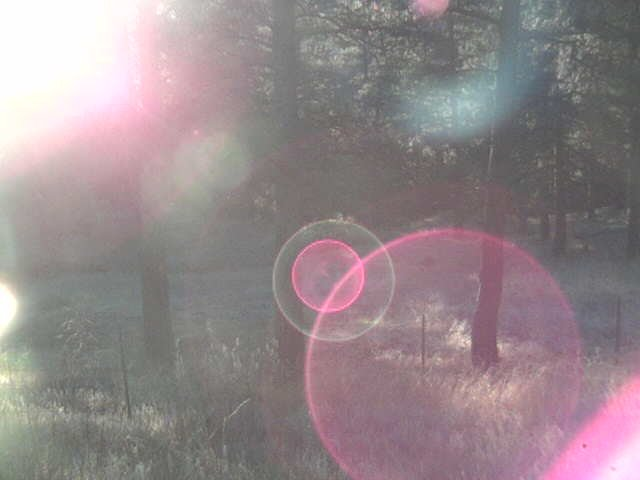
\includegraphics[width=0.45\linewidth, keepaspectratio]{figures/CCTV-Lens-flare.jpg}
}%
\subfigure[Vignetting\newline Image by \cite{image:wikipedia:vignetting}]{
  \label{fig:Vignetting}
  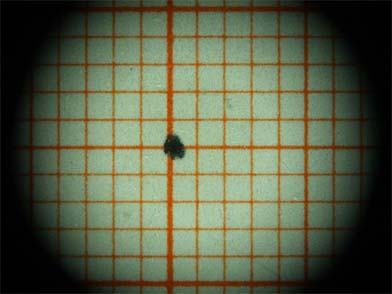
\includegraphics[width=0.45\linewidth, keepaspectratio]{figures/Randabschattung-Mikroskop-Kamera-6.JPG}
}
\subfigure[Smoke\newline Image by \cite{giannarou2013probabilistic}]{
  \label{fig:smoke}
  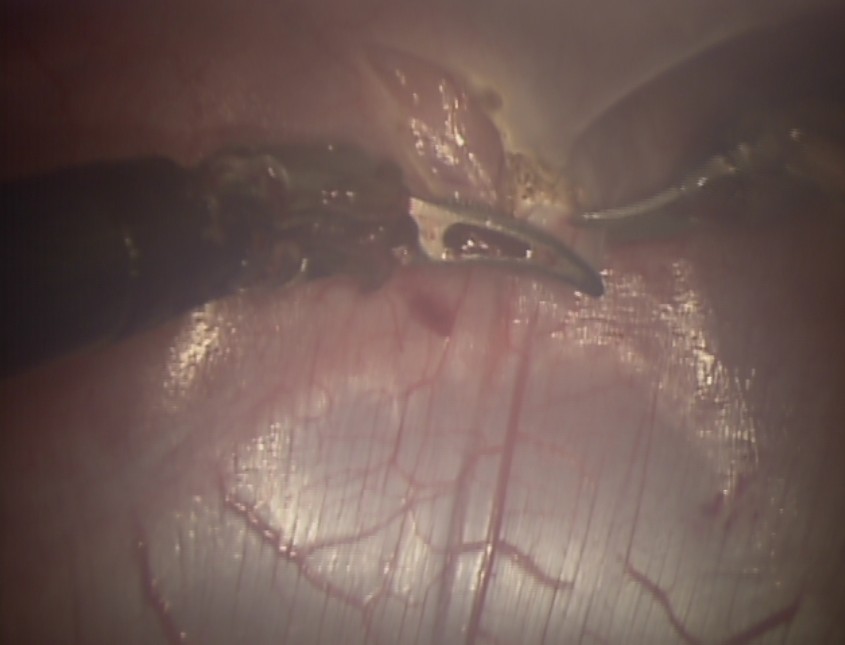
\includegraphics[width=0.45\linewidth, keepaspectratio]{figures/smoke-capture1-033.png}
}%
\subfigure[Camouflage\newline Image by \cite{image:wikipedia:camouflage}]{
  \label{fig:camouflage}
  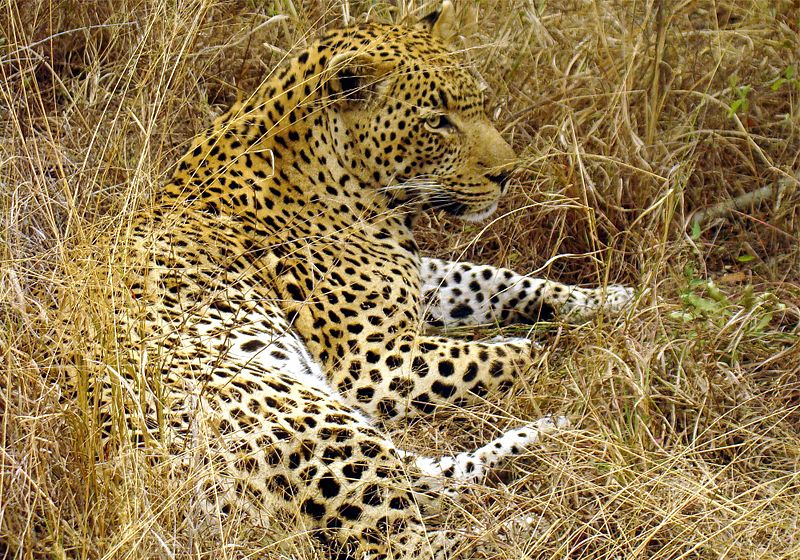
\includegraphics[width=0.45\linewidth, keepaspectratio]{figures/great-male-leopard.JPG}
}
\subfigure[Transparency]{
  \label{fig:transparency-glass}
  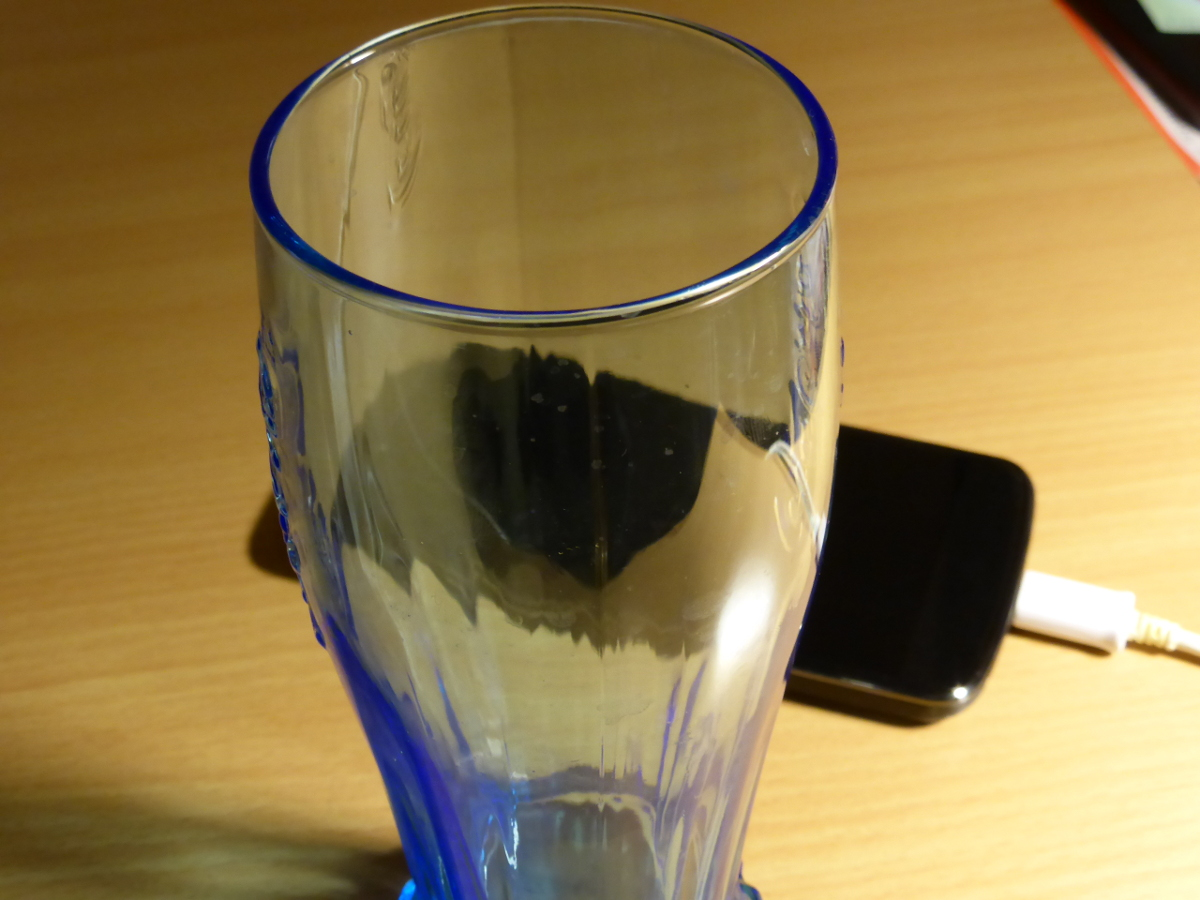
\includegraphics[width=0.45\linewidth, keepaspectratio]{figures/glass-smartphone-table-2.jpg}
}%
\subfigure[Viewpoint]{
  \label{fig:viewpoint}
  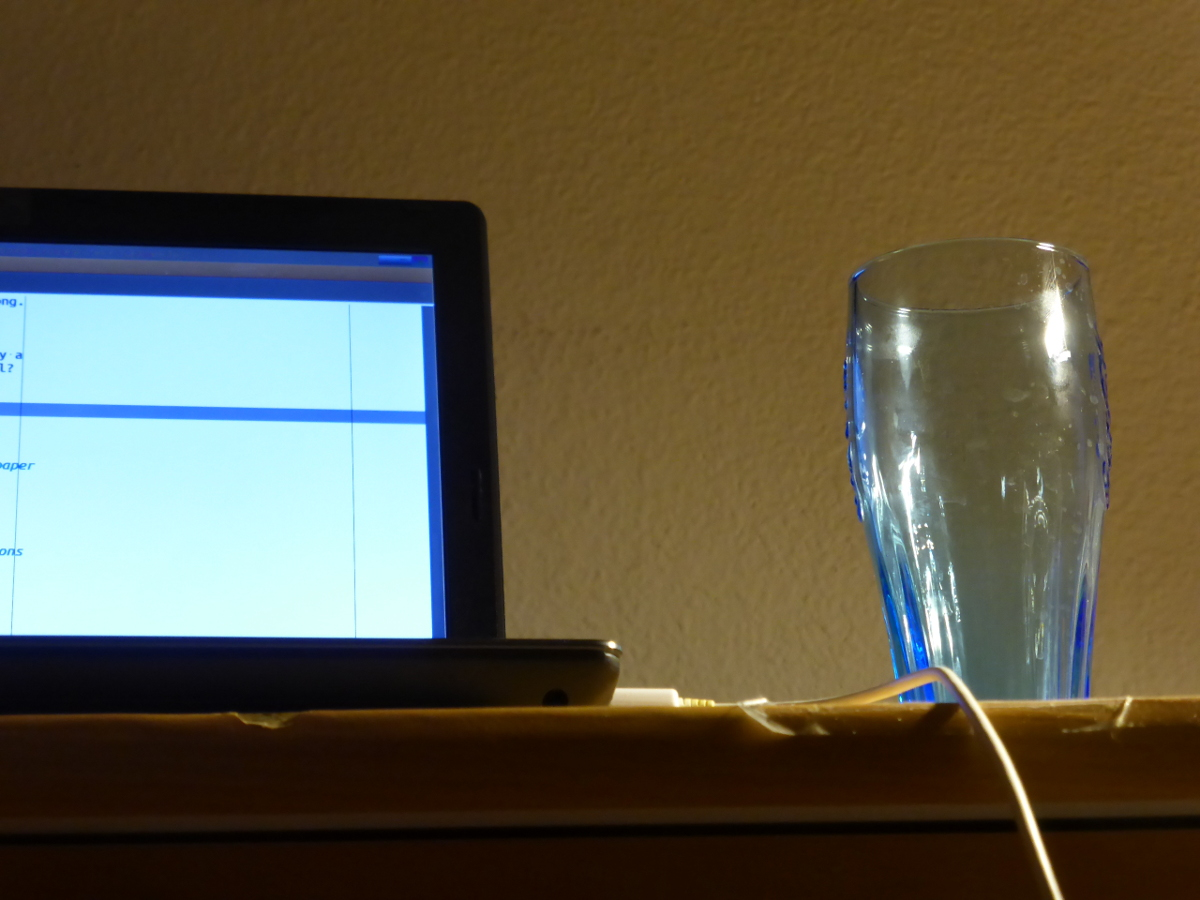
\includegraphics[width=0.45\linewidth, keepaspectratio]{figures/unusual-viewpoint-glass-computer.jpg}
}
\caption{Examples of images which might cause semantic segmentation systems to fail.}
\label{fig:test}
\end{figure}


\subsection{Unsharp images}
Images can be unsharp for a couple of reasons. A problem with the lenses
machanics, focusing on the wrong point, too quick movement, smoke or foam.
One example of an unsharp image is \cref{fig:smoke}, which was taken during an
in~vivo porcine procedure of diaphragm dissection. The smoke was caused by
cauterisation.


\subsection{Other Problems}
If the following effects can occur at all and if they are problems depends
heavily on the problem domain and the used model.

\subsubsection{Partial Occlusions}
Segmentation systems which employ a model of the objects which should be
segmented might suffer from partial occlusions.

\subsubsection{Camouflage}
Some objects, like animals in the wild, actively try to hide
(see~\cref{fig:camouflage} as an example). In other cases it might just be bad
luck that objects are hard for humans to detect. This problem has two
interesting aspects: On the one hand, the segmenting system might suffer from
the same problems as humans do. On the other hand, the segmenting system might
be better than humans are, but it is forced to learn from images labeled by
humans. If the labels are wrong, the system is forced to learn something wrong.

\subsubsection{Semi-transparent Occlusion}
Some objects like drinking glasses can be visible and still leave the object
behind them visible as shown in \cref{fig:transparency-glass}. This is mainly a
definition problem: Is the seen pixel the glass label or the smartphone label?

\subsubsection{Viewpoints}
Changes in viewpoints can be a problem, if they don't occur in the training
data. For example, an image captioning system which was trained on photographs
of professional photographers might not have photos from the point of view of
a child. This is visualized in \cref{fig:viewpoint}.

% \subsubsection{Strong Contrast}
% Strong contrast on the same object, e.g. butterflies or printed pieces of paper
% https://commons.wikimedia.org/wiki/File:Nymphalis_io_Luc_Viatour.jpg


% \begin{itemize}
% %    \item reflections - https://commons.wikimedia.org/wiki/Category:Reflections
%     % https://commons.wikimedia.org/wiki/File:Light_through_glass.jpg
%     % https://commons.wikimedia.org/wiki/Glass
% \end{itemize}
